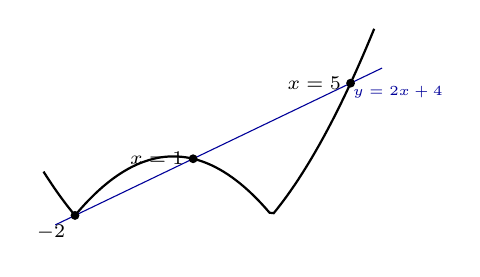
\begin{tikzpicture}[x=5mm,y=1.2mm]
\ax{-3}{6.5}{-1}{15.5}
\draw[thick,domain=-2.8:5.6,samples=80] plot (\x,{abs((\x)^2-\x-6)});
\draw[blue!60!black,domain=-2.5:5.8,samples=80] plot (\x,{2*\x+4});
\fill (-2,0) circle (1.6pt);
\node[below left] at (-2,0){\scriptsize $-2$};
\fill (1,6) circle (1.6pt);
\node[left] at (1,6){\scriptsize $x=1$};
\fill (5,14) circle (1.6pt);
\node[left] at (5,14){\scriptsize $x=5$};
\node[blue!60!black] at (6.2,13){\tiny $y=2x+4$};
\end{tikzpicture}